\documentclass{lab_sheet}
\usepackage[flushleft]{threeparttable}
\usepackage[hidelinks]{hyperref}
\newcommand{\activitypingpc}[1]{
    \cmdop{#1-a}{ping test from PC1 to PC2}
    \cmdop{#1-b}{ping test from PC2 to PC3}
    \cmdop{#1-c}{ping test from PC3 to PC4}
    \cmdop{#1-d}{ping test from PC4 to PC1}
    \cmdop{#1-e}{ping test from PC1 to PC3}
    \cmdop{#1-f}{ping test from PC2 to PC4}
}

\newcommand{\setting}[2]{
    \begin{tabular}{C{3cm}C{4cm}}
        \toprule
          #1 & IP address \\
          \midrule
          #2
          \bottomrule
       \end{tabular}
}


\newcommand{\subnets}[1]{
    \begin{tabular}{C{3cm}C{6cm}}
        \toprule
          Network Address & Usable  IP addresses \\
          \midrule
          #1
          \bottomrule
       \end{tabular}
}

\begin{document}
    \titlePage{To Introduce the Concept of Subnetting, Subnet Mask, VLSM \& CIDR}{December 3, 2020}
    \pagenumbering{gobble}
    \tableofcontents
    \pagebreak
    \listoffigures
    \pagebreak
    \listoftables
    \pagebreak
    \lstlistoflistings
    \pagebreak
    \pagenumbering{arabic}
    \section{Objectives}
    \begin{itemize}
        \item Familiarization with subnetting, subnet mask and its use.
        \item Familiarization with VLSM and CIDR.
    \end{itemize}
    \section{Required Tools}
    \subsection{Cisco Packet Tracer}
    Cisco Packet Tracer is a visual simulation software developed and distributed by Cisco Systems. Packet Tracer is a cross platform tool that allows simulated environment for modern computer network and network topologies.
    \section{Simulation Activities}
    \begin{figure}[H]
        \centering
        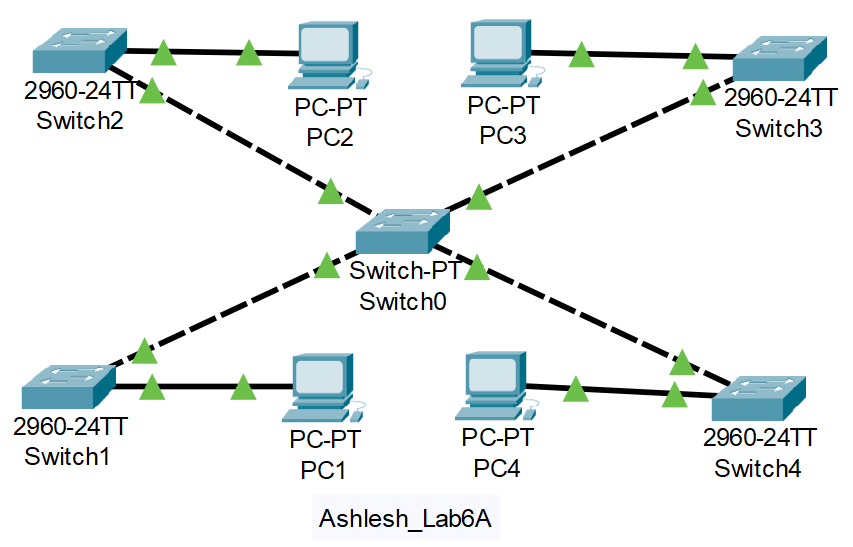
\includegraphics[scale=.5]{Figures/activitya.png}
        \caption{Simulated network for Activity A and C}
        \label{fig:activitya}
    \end{figure}

    \begin{figure}[H]
      \centering
      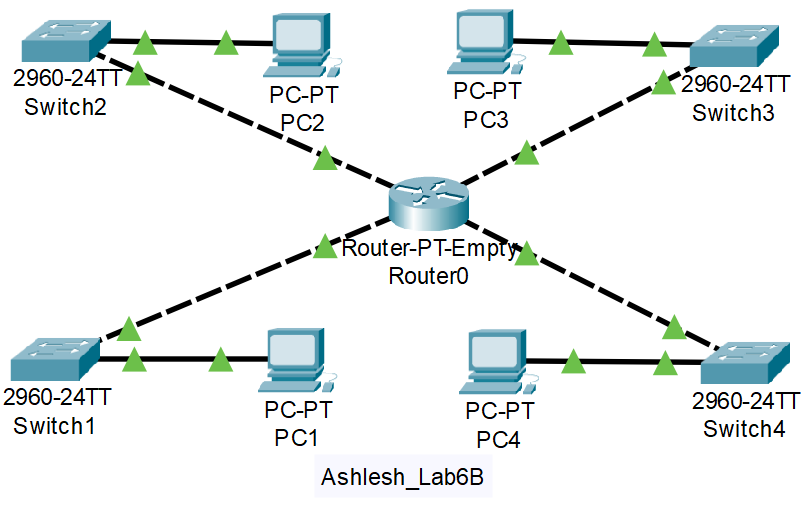
\includegraphics[scale=.5]{Figures/activityb.png}
      \caption{Simulated network for Activity B}
      \label{fig:activityb}
  \end{figure}

  \begin{figure}[H]
    \centering
    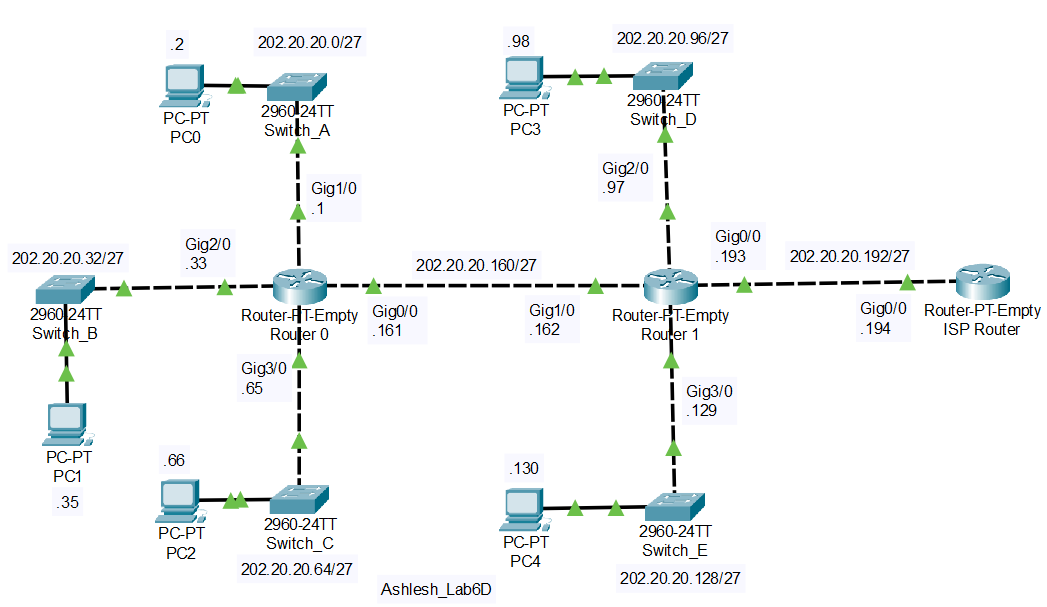
\includegraphics[scale=.7]{Figures/activityd.png}
    \caption{Simulated network for Activity D}
    \label{fig:activityd}
\end{figure}

\begin{figure}[H]
    \centering
    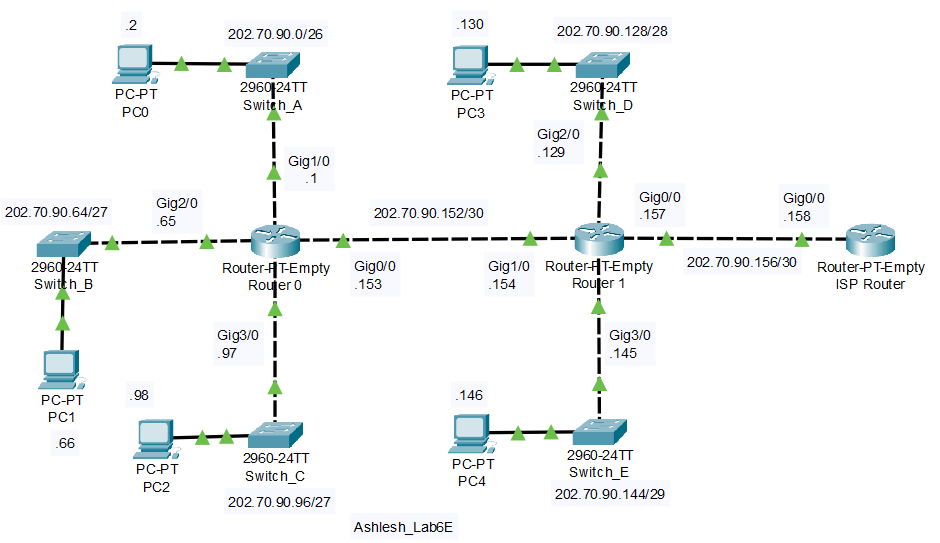
\includegraphics[scale=.75]{Figures/activitye.png}
    \caption{Simulated network for Activity E}
    \label{fig:activitye}
\end{figure}

    \section{Exercises}
\problem{Observe and note down the output of each of the mentioned tasks from the lab sheet and comment on the result by explaining the reason in detail.}
\subproblem{Activity A}
\addtocontents{lol}{\protect\subsection*{Activity A}}
\addtocontents{lot}{\protect\subsection*{Activity A}}
\subsubsection*{Sub activity 1}
\addtocontents{lot}{\protect\subsubsection*{Sub activity 1}}
The network shown in Figure~\ref{fig:activitya} is created using Packet Tracer with basic settings as,
    \begin{table}[H]
        \centering
        \setting{PC}{
        1 & 202.22.22.11   \\
        2 & 202.22.22.21  \\
        3 & 202.22.22.41   \\
        4 & 202.22.22.81   \\
        }
  \caption{IP address for the PCs in the network}
  \label{tbl:pcsettinga}
\end{table}
\subsubsection*{Sub activity 2}
\addtocontents{lol}{\protect\subsubsection*{Sub activity 2}}
The subnet mask for all the PCs is set to 255.255.255.0.
\activitypingpc{a2}
The subnet mask /24 means that the network has usable hosts in the range 202.22.22.0 to 202.22.22.254, which is why all the ping request complete successfully.
\subsubsection*{Sub activity 3}
\addtocontents{lol}{\protect\subsubsection*{Sub activity 3}}
\addtocontents{lot}{\protect\subsubsection*{Sub activity 3}}
The subnet mask for all the PCs is set to 255.255.255.192.
\activitypingpc{a3}
\begin{table}[H]
    \centering
    \subnets{
        202.22.22.0 & 202.22.22.1 - 202.22.22.62 \\
        202.22.22.64 & 202.22.22.65 - 202.22.22.126 \\
        202.22.22.128 & 202.22.22.129 - 202.22.22.190 \\
        202.22.22.192 & 202.22.22.193 - 202.22.22.254 \\
}
\caption{Possible /26 networks for 202.22.22.*}
\label{tbl:a3}
\end{table}
The subnet mask /26 means that the network is divided into 4 subnets as shown in Table~\ref{tbl:a3}. This means that PC1, PC2 and PC3 are in the same network, 202.22.22.0 and PC4 is in the subnet 202.22.22.65, which is why the ping request to and from PC4 to other PCs fail.

\subsubsection*{Sub activity 4}
\addtocontents{lol}{\protect\subsubsection*{Sub activity 4}}
\addtocontents{lot}{\protect\subsubsection*{Sub activity 4}}
The subnet mask for all the PCs is set to 255.255.255.224.
\activitypingpc{a4}
\begin{table}[H]
    \centering
    \subnets{
        202.22.22.0 & 202.22.22.1 - 202.22.22.30 \\
        202.22.22.32 & 202.22.22.33 - 202.22.22.62 \\
        202.22.22.64 & 202.22.22.65 - 202.22.22.94 \\
        202.22.22.96 & 202.22.22.97 - 202.22.22.126 \\
        202.22.22.128 & 202.22.22.129 - 202.22.22.158 \\
        202.22.22.160 & 202.22.22.161 - 202.22.22.190 \\
        202.22.22.192 & 202.22.22.193 - 202.22.22.222 \\
        202.22.22.224 & 202.22.22.225 - 202.22.22.254 \\
}
\caption{Possible /27 networks for 202.22.22.*}
\label{tbl:a4}
\end{table}
The subnet mask /27 means that the network is divided into 8 subnets as shown in Table~\ref{tbl:a4}. This means that PC1 and PC2 are in the same network, 202.22.22.0. PC3 is in the subnet 202.22.22.32 whereas PC4 is in the subnet 202.22.22.65, which is why the ping request to and from PCs in different subnet fails.

\subsubsection*{Sub activity 5}
\addtocontents{lol}{\protect\subsubsection*{Sub activity 5}}
\addtocontents{lot}{\protect\subsubsection*{Sub activity 5}}
The subnet mask for all the PCs is set to 255.255.255.240.
\activitypingpc{a5}
\begin{table}[H]
    \centering
    \subnets{
        202.22.22.0 & 202.22.22.1 - 202.22.22.14 \\
        202.22.22.16 & 202.22.22.17 - 202.22.22.30 \\
        202.22.22.32 & 202.22.22.33 - 202.22.22.46 \\
        202.22.22.48 & 202.22.22.49 - 202.22.22.62 \\
        202.22.22.64 & 202.22.22.65 - 202.22.22.78 \\
        202.22.22.80 & 202.22.22.81 - 202.22.22.94 \\
        202.22.22.96 & 202.22.22.97 - 202.22.22.110 \\
        202.22.22.112 & 202.22.22.113 - 202.22.22.126 \\
        202.22.22.128 & 202.22.22.129 - 202.22.22.142 \\
        202.22.22.144 & 202.22.22.145 - 202.22.22.158 \\
        202.22.22.160 & 202.22.22.161 - 202.22.22.174 \\
        202.22.22.176 & 202.22.22.177 - 202.22.22.190 \\
        202.22.22.192 & 202.22.22.193 - 202.22.22.206 \\
        202.22.22.208 & 202.22.22.209 - 202.22.22.222 \\
        202.22.22.224 & 202.22.22.225 - 202.22.22.238 \\
        202.22.22.240 & 202.22.22.241 - 202.22.22.254 \\
}
\caption{Possible /28 networks for 202.22.22.*}
\label{tbl:a5}
\end{table}
The subnet mask /28 means that the network is divided into 8 subnets as shown in Table~\ref{tbl:a5}. This means that all the PCs are in different subnets which is why the ping test to and from any PC to other PCs fails.

\subproblem{Activity B}
\addtocontents{lol}{\protect\subsection*{Activity B}}
\addtocontents{lot}{\protect\subsection*{Activity B}}
The network shown in Figure~\ref{fig:activityb} is created using Packet Tracer with basic settings for the gigabitethernet interfaces as,
    \begin{table}[H]
        \centering
        \setting{Gigabitethernet interfaces}{
        0/0 & 202.22.22.1   \\
        1/0 & 202.22.22.17  \\
        2/0 & 202.22.22.33   \\
        3/0 & 202.22.22.82   \\
        }
  \caption{IP address for the gigabitethernet interfaces of the router in the network}
  \label{tbl:gigasettingb}
\end{table}
The subnet mask for all the PCs is set to 255.255.255.240. The default gateway for PC1, PC2, PC3 and PC4 are set as 202.22.22.1, 202.22.22.17, 202.22.22.33 and 202.22.22.82 respectively. 
\activitypingpc{b}
Although the PCs are in different subnets due to the /28 subnet mask, the set default gateways and routing capabilities of the router connected instead of the switch make sure the packets are properly passed on and hence the ping tests succeed.
\subproblem{Activity C}
\addtocontents{lol}{\protect\subsection*{Activity C}}
\addtocontents{lot}{\protect\subsection*{Activity C}}
The network shown in Figure~\ref{fig:activitya} is created using Packet Tracer with basic settings as,
    \begin{table}[H]
        \centering
        \setting{PC}{
        1 & 202.44.8.2   \\
        2 & 202.44.9.2  \\
        3 & 202.44.10.2   \\
        4 & 202.44.11.2  \\
        }
  \caption{IP address for the PCs in the network}
  \label{tbl:pcsettingc}
    \end{table}
\subsubsection*{Sub activity 1}
\addtocontents{lol}{\protect\subsubsection*{Sub activity 1}}
The subnet mask for all the PCs is set to 255.255.255.0.
\activitypingpc{c1}
The subnet mask /24 means that the PCs underconsideration are all under different subnets. PC1, PC2, PC3 and PC4 are in 202.44.8.0, 202.44.9.0, 202.44.10.0 and 202.44.11.0 networks respectively, which is why the ping test to and from any PC to other PCs fails.
\subsubsection*{Sub activity 2}
\addtocontents{lol}{\protect\subsubsection*{Sub activity 2}}
The subnet mask for all the PCs is set to 255.255.254.0.
\activitypingpc{c2}
The subnet mask /23 means that PC1 and PC2 are in 202.44.8.0 network and PC3 and PC4 are in 202.44.10.0 network, which is why the ping test to and from any PC to other PCs outside its subnet fails.
\subsubsection*{Sub activity 3}
\addtocontents{lol}{\protect\subsubsection*{Sub activity 3}}
The subnet mask for all the PCs is set to 255.255.252.0.
\activitypingpc{c3}
The subnet mask /22 means that the PCs underconsideration are all under same subnet, i.e. 202.44.8.0, which is why the ping test to and from any PC to other PCs succeds.
\subsubsection*{Sub activity 4}
\addtocontents{lol}{\protect\subsubsection*{Sub activity 4}}
The subnet mask for all the PCs is set to 255.255.248.0.
\activitypingpc{c4}
The subnet mask /21 means that the PCs underconsideration are all under same subnet, i.e. 202.44.8.0, which is why the ping test to and from any PC to other PCs succeds.
\subproblem{Activity D}
\addtocontents{lot}{\protect\subsection*{Activity D}}
The main network as provided by the ISP is 202.20.20.0/24, which means there are 254 possible hosts within the network. The requirement as set by the problem is that all the 7 subnets need to have equal range. For this, all the subnets are provided with 30 hosts each, which means we need to use /27 as the subnet mask for each subnet. \\[\baselineskip]
Figure~\ref{fig:activityd} shows the topology created using packet tracer where each department is represented by a switch having only one host for simulation purposes. Subnets A, B and C are connected to the Router 0 with required IP address and subnet mask in PC0, PC1, PC2, gigabitethernet interfaces 1/0, 2/0 and 3/0. Gigabitethernet interface 0/0 of the Router 0 is connected with gigabitethernet interface 1/0 of Router 1 in the network 202.20.20.160/27. Likewise,subnets D and E are connected to the Router 1 with required IP address and subnet mask in PC3, PC4, gigabitethernet interfaces 1/0, 2/0 and 3/0. Gigabitethernet interface 0/0 of the Router 1 is connected with gigabitethernet interface 0/0 of ISP Router in the network 202.20.20.192/27.\\[\baselineskip]
For routing purposes, default route is configured in Router 0 such that the next hop is the gigabitethernet interface 1/0 of Router 1. Likewise, static routes for networks 202.20.20.0/27, 202.20.20.32/27 and 202.20.20.64/27 are set in Router 1 with the next hop as the gigabitethernet interface 0/0 on Router 0. Similarly, the default route in Router 1 is set such that the next hop is the gigabitethernet interface 0/0 on ISP Router. Finally, static routes for all the subnets A, B, C, D and E are set for ISP Router with gigabitethernet interface 0/0 of Router 1 being the next hop.\\[\baselineskip]
Since using the ping program on this network would be a lengthy process, the connectivity was tested using simple PDUs within the packet tracer program which gave the following results.
\begin{figure}[H]
    \foreach \x in {0,1,2,3}
    {
        \begin{subfigure}{.5\textwidth}
            \centering
            \includegraphics[width=.8\linewidth,frame]{Figures/d-\x.png}
            \caption{Observation for connectivity test from PC\x~to other PCs and routers}
            \label{fig:d-\x}
        \end{subfigure}
    }
      \hspace*{\fill}
      \begin{subfigure}{.5\textwidth}
        \centering
        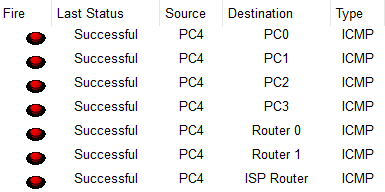
\includegraphics[width=.8\linewidth,frame]{Figures/d-4.png}
        \caption{Observation for connectivity test from PC4 to other PCs and routers}
        \label{fig:d-4}
      \end{subfigure}
      \hspace*{\fill}
    \caption{Observation for connectivity test in activity D}
    \label{fig:obs-d}
\end{figure}

\begin{table}[H]
    \centering
    \begin{tabular}{|C{1cm}||C{2cm}||C{2.5cm}||C{5cm}||C{1cm}|}
     \hline
     Subnet&Required Hosts&Network Address&
     Usable IP Addresses&Subnet Mask\\
     \hline
     A & 30 & 202.20.20.0 &  202.20.20.1~-~202.20.20.30 & /27\\
     \hline
     B & 30 & 202.20.20.32 & 202.20.20.33~-~202.20.20.62 & /27\\
     \hline
     C & 30 & 202.20.20.64 & 202.20.20.65~-~202.20.20.94 & /27\\
     \hline
     D & 30 & 202.20.20.96 & 202.20.20.97~-~202.20.20.126 & /27\\
     \hline
     E & 30 & 202.20.20.128 & 202.20.20.129~-~202.20.20.158 & /27\\
     \hline
     F & 30 & 202.20.20.160 &  202.20.20.161~-~202.20.20.19 & /27\\
     \hline
     G & 30 & 202.20.20.192 & 202.20.20.193~-~202.20.20.222 & /27\\
     \hline
    \end{tabular}
    \caption{Subnet division as required by activity D}
    \label{tbl:activityd}
    \end{table}

\subproblem{Activity E}
\addtocontents{lot}{\protect\subsection*{Activity E}}
The main network as provided by the ISP is 202.70.90.0/24, which means there are 254 possible hosts within the network. The requirement as set by the problem is that department A, B, C, D and E need 54, 27, 18, 12 and 6 hosts respectively. Likewise, there are two point to point connections needed between the routers. For this, the main network is subnetted using VLSM, which means we need to use different subnet mask for each subnet resulting in appropriate number of hosts. \\[\baselineskip]
Figure~\ref{fig:activitye} shows the topology created using packet tracer where each department is represented by a switch having only one host for simulation purposes. Subnets A, B and C are connected to the Router 0 with required IP address and subnet mask in PC0, PC1, PC2, gigabitethernet interfaces 1/0, 2/0 and 3/0. Gigabitethernet interface 0/0 of the Router 0 is connected with gigabitethernet interface 1/0 of Router 1 in the network 202.70.90.152/30. Likewise,subnets D and E are connected to the Router 1 with required IP address and subnet mask in PC3, PC4, gigabitethernet interfaces 1/0, 2/0 and 3/0. Gigabitethernet interface 0/0 of the Router 1 is connected with gigabitethernet interface 0/0 of ISP Router in the network 202.70.90.156/30.\\[\baselineskip]
For routing purposes, default route is configured in Router 0 such that the next hop is the gigabitethernet interface 1/0 of Router 1. Likewise, static routes for networks 202.70.90.0/26, 202.70.90.64/27 and 202.70.90.96/27 are set in Router 1 with the next hop as the gigabitethernet interface 0/0 on Router 0. Similarly, the default route in Router 1 is set such that the next hop is the gigabitethernet interface 0/0 on ISP Router. Finally, static routes for all the subnets A, B, C, D and E are set for ISP Router with gigabitethernet interface 0/0 of Router 1 being the next hop.\\[\baselineskip]
The connectivity was tested using simple PDUs within the packet tracer program which gave the following results.
\begin{figure}[H]
    \foreach \x in {0,1}
    {
        \begin{subfigure}{.5\textwidth}
            \centering
            \includegraphics[width=.8\linewidth,frame]{Figures/d-\x.png}
            \caption{Observation for connectivity test from PC\x~to other PCs and routers}
            \label{fig:e-\x}
        \end{subfigure}
    }
    \caption{Observation for connectivity test in activity E}
    \label{fig:obs-e}
\end{figure}

\begin{figure}[H]\ContinuedFloat
    \foreach \x in {2,3}
    {
        \begin{subfigure}{.5\textwidth}
            \centering
            \includegraphics[width=.8\linewidth,frame]{Figures/d-\x.png}
            \caption{Observation for connectivity test from PC\x~to other PCs and routers}
            \label{fig:e-\x}
        \end{subfigure}
    }
\hspace*{\fill}
\begin{subfigure}{.5\textwidth}
  \centering
  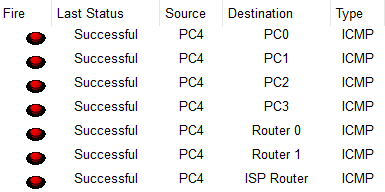
\includegraphics[width=.8\linewidth,frame]{Figures/d-4.png}
  \caption{Observation for connectivity test from PC4 to other PCs and routers}
  \label{fig:e-4}
\end{subfigure}
\hspace*{\fill}
    \caption*{Figure~\ref{fig:obs-e}:~Observation for connectivity test in activity E (continued)}
\end{figure}

\begin{table}[H]
    \centering
    \begin{tabular}{|C{1cm}||C{2cm}||C{2.5cm}||C{5cm}||C{1cm}|}
     \hline
     Subnet&Required Hosts&Network Address&
     Usable IP Addresses&Subnet Mask\\
     \hline
     A & 54 & 202.70.90.0 &  202.70.90.1~-~202.70.90.62 & /26\\
     \hline
     B & 27 & 202.70.90.64 & 202.70.90.65~-~202.70.90.94 & /27\\
     \hline
     C & 18 & 202.70.90.96 & 202.70.90.97~-~202.70.90.126 & /27\\
     \hline
     D & 12 & 202.70.90.128 & 202.70.90.129~-~202.70.90.142 & /28\\
     \hline
     E & 6 & 202.70.90.144 & 202.70.90.145~-~202.70.90.150 & /29\\
     \hline
     F & 2 & 202.70.90.152 &  202.70.90.153~-~202.70.90.154 & /30\\
     \hline
     G & 2 & 202.70.90.156 & 202.70.90.157~-~202.70.90.158 & /30\\
     \hline
    \end{tabular}
    \caption{Subnet division as required by activity E}
    \label{tbl:activitye}
    \end{table}

    \problem{Explain subnetting and VLSM with their importance in networking with suitable examples.}
    Subnetting is a logical process by which a larger TCP/IP network is divided or subnetted into smaller networks called subnets for easy management purposes. It is achieved using a four octet or 32-bit number called a subnet mask.
    There are mainly two types of subnet masks by which subnetting can be achieved, viz. FLSM and VLSM. If all the subnets in a larger network have equal number of hosts it is said to be using FLSM, whereas subnets with different number of hosts are said to be using VLSM.
    \\[\baselineskip]
     Consider an organization, for instance say a campus that has access to a private network given by the address 192.168.1.0/24 which means that there are 254 available IP addresses in the major network. If there are three departments that need IP addresses to assign to host devices within the department and we wish to provide separate subnets to each of the departments, we can achieve this with a subnet mask 255.255.255.192, i.e. /26 in slash notation. This divides the main network 192.168.1.0/24 into three subnets namely A, B and C. Each of these subnets has 62 possible host IP addresses, one network address each as 192.168.1.0, 192.168.1.64 and 192.168.1.128 and one broadcast address each as 192.168.1.63, 192.168.1.127 and 192.168.1.191 respectively. This essentially divides the main network into separate subnets with separate management capabilities. This also reduces network congestion with network traffic being isolated in the subnet that it originated in, but still providing a cross subnet communication. \\[\baselineskip]
     Similarly, VLSM provides the capability of each subnet having varying number of hosts. This ensures that each department gets the needed amount of hosts but doesn't over occupy the IP addresses from the main network.

     \problem{What is classless routing? Why is it used in Internet system? Explain with suitable examples.}
     Classless routing protocols are one that send the subnet mask along with their updates. This allows classless routing to support both route summarization and VLSM. When the destination of a packet only matches the defualt route and no other routes, then the packet is forwarded using the default route. Classless routing also supports CIDR (Classless Inter-Domain Routing), which is a method of assigning IP address to improve distribution. \\[\baselineskip]
     For the three classes of a classful network,
     \begin{itemize}
         \item Class A supports over 16 million identifiers
         \item Class B supports 65535 identifiers
         \item Class C supports 254 identifiers
     \end{itemize}
     Whenever an organization requires over 254 hosts, traditionally it would have to switch to a class B network. However, not all identifiers would be used sensibly and it causes inefficiency in address assigning. Since CIDR is based on VLSM, the network can be subnetted to provide the required number of hosts and prevent the wastage of IP addresses. It also allows only one entry in the routing table for the supernet to represent the overall network which reduces the table's size.

     \section{Conclusion}
     The activities provided in the lab sheet were performed which aided in understanding the concept of subnetting in more detail, subnet masks and their impact on a network subnet, VLSM to divide a network into subnets with different number of hosts and CIDR. While performing activity A, the concept of subnet mask and its impact on subnetting was understood. Although initially the PCs were on the same network, once the subnet mask was gradually changed, the PCs began to get separated in different subnets. This way the ping tests from PCs in different subnets failed. Similarly, in activity B, similar network was connected using a router with default gateways set properly. So, although the PCs were in different subnets, the ping tests succeeded since the router properly routed the packets due to the proper gateways on the PCs. Likewise, in activity C, initially the PCs were in different subnets. Gradually changing the subnet masks in the sub activities, we could see the PCs getting into a single network as the range of individual subnets were getting increased. Finally all the PCs were in same subnet and hence the ping succeeded. For activity D, we created a complex network topolgy with 7 subnets all having the same number of host devices. This was clearly an introdcution as to how IP addresses were wasted while using FLSM. In activity E, similar network with departments needing different number of hosts was created. This was possible due to the application of VLSM. The routes for both the activity D and E were set such that all PCs were connected to each other through either staic or default routes as discussed in previous lab experiments. The completion of this lab experiment allowed us to be familiar with the concepts of subnetting, subnet masks, VLSM and CIDR.
     \end{document}
